% !TEX program = xelatex
\documentclass[conference]{IEEEtran}

% Required packages
\usepackage{graphicx}
\usepackage{listings}
\usepackage{xcolor}
\usepackage{url}
\usepackage{fontspec}
\usepackage{fvextra}
\usepackage{amsmath}
\usepackage{amssymb}
\usepackage{newunicodechar}

% Times-compatible main font and a monospace font with
% box-drawing characters used in the AI transcripts
\setmainfont{texgyretermes}[
    Extension=.otf,
    UprightFont=*-regular,
    BoldFont=*-bold,
    ItalicFont=*-italic,
    BoldItalicFont=*-bolditalic
]
\setmonofont{DejaVuSansMono}[
    Extension=.ttf,
    BoldFont=*-Bold,
    ItalicFont=*-Oblique,
    BoldItalicFont=*-BoldOblique,
    Scale=MatchLowercase
]

% Emoji in the transcripts that no installed font provides
\newunicodechar{✅}{[OK]}
\newunicodechar{❌}{[X]}

% Source code formatting
\lstset{
    basicstyle=\ttfamily\scriptsize,
    breaklines=true,
    breakatwhitespace=false,
    frame=single,
    numbers=left,
    numberstyle=\tiny,
    numbersep=4pt,
    showstringspaces=false,
    columns=fullflexible,
    keepspaces=true
}

% Report title
\title{Applications of Greedy and
Divide-and-Conquer Algorithms}

\author{
    \IEEEauthorblockN{Group Project}
}

\begin{document}

\maketitle

% Introduction
\section{Introduction}

This report examines the application of
greedy and divide-and-conquer algorithms
to real-world computational problems.

Both problems are drawn from traffic signal
operations. The greedy section selects a maximum
set of compatible green-light windows, and the
divide-and-conquer section identifies the period
of worst queue build-up on an intersection
approach from detector counts.

% =====================================
% GREEDY ALGORITHM
% =====================================

\section{Greedy Algorithm:
Traffic Signal Scheduling}

\subsection{Real-World Problem Description}

Traffic congestion is a common problem in urban
areas, particularly at intersections controlled
by traffic signals. Poorly coordinated traffic
signals can cause vehicles to stop repeatedly,
increase waiting times, and contribute to
congestion along major roads.

One issue occurs when traffic signals release
vehicles from one intersection while another
intersection farther down the road is unable
to accommodate the incoming traffic.

This problem motivated the investigation of
traffic signal scheduling using a greedy
algorithm.

For this project, we consider a simplified
traffic signal scheduling problem.

A traffic management system is assumed to
provide a collection of candidate green-light
time windows for a particular traffic movement.

Each window represents a time interval during
which a green-light opportunity could be
scheduled.

The scheduling system must select a subset
of these windows such that no two selected
windows overlap.

The objective is to maximize the total
number of compatible green-light windows.

This simplified model assumes that all
candidate windows have equal importance,
each window is indivisible, and the safety
and feasibility of every candidate window
have already been verified.

Although real-world traffic signal
coordination involves additional factors,
including traffic volume, vehicle speeds,
pedestrian crossings, and intersection
capacity, this abstraction allows us
to study an optimization problem that
can be solved optimally using a
greedy algorithm.

Traffic signal coordination is used to synchronize
intersections to improve traffic progression and
reduce unnecessary stops and delays \cite{fhwa2008}.

\subsection{Mathematical Abstraction}

The traffic signal scheduling problem
is modeled as a set of time intervals.

Let

\[
W = \{w_1, w_2, \ldots, w_n\}
\]

represent the set of candidate green-light
windows.

Each window is represented as

\[
w_i = (s_i, f_i)
\]

where:

\begin{itemize}
    \item $s_i$ represents the starting
    time of window $i$.

    \item $f_i$ represents the finishing
    time of window $i$.

    \item $n$ represents the total number
    of candidate windows.
\end{itemize}

Every window must satisfy

\[
s_i < f_i.
\]

Two windows are compatible when they
do not overlap.

For two windows $w_i$ and $w_j$,
where $w_i$ is scheduled before $w_j$,
compatibility requires

\[
f_i \leq s_j.
\]

This means that the next window may
begin only after the previous
selected window has finished.

The goal is to find a subset

\[
S \subseteq W
\]

that maximizes the number of
selected windows:

\[
\max |S|
\]

subject to the constraint that
all selected windows are
mutually compatible.

This is a maximum-cardinality
interval scheduling problem.

The greedy algorithm solves this
problem by sorting candidate
windows according to their
finishing times and repeatedly
selecting the earliest-finishing
window that does not conflict
with previously selected windows.

The result is an optimal subset
containing the maximum possible
number of compatible green-light
windows under the stated assumptions.
\subsection{Greedy Algorithm Design}

The algorithm uses the earliest-finish-time greedy
strategy. It sorts the candidate windows in ascending
order of finishing time, then scans them in that order,
selecting a window if it starts no earlier than the
finish of the previously selected window and skipping
it otherwise.

\subsubsection{Algorithm Pseudocode}

\begin{verbatim}
GREEDY-WINDOW-SCHEDULING(W)
Input:  W = candidate green-light windows
Output: S = maximum set of compatible windows

1. Sort W by ascending finishing time
2. S = empty list;  lastFinish = -infinity
3. for each window w in W:
4.     if w.start >= lastFinish:
5.         add w to S;  lastFinish = w.finish
6. return S
\end{verbatim}

\subsubsection{Greedy Choice}

The greedy choice is the compatible window with the
earliest finishing time: finishing earlier leaves at
least as much time for later windows as any other
choice. Its optimality is proved by an exchange
argument in Section~\ref{sec:greedy-proof}.

\subsubsection{Explanation in the Traffic Signal Domain}

Each candidate window is a period in which a traffic
movement could receive a green signal. The scheduling
system arranges these opportunities by ending time,
approves the earliest-ending one, and then approves
each subsequent opportunity only if it does not overlap
an already approved green-light window.

For example, consider the following windows:

\begin{center}
\begin{tabular}{|c|c|c|}
\hline
Window & Start (s) & Finish (s) \\
\hline
1 & 0 & 10 \\
2 & 2 & 5 \\
3 & 5 & 8 \\
4 & 7 & 12 \\
5 & 8 & 14 \\
\hline
\end{tabular}
\end{center}

After sorting by finishing time, the algorithm selects
window 2 (finishing at 5\,s), window 3 (starting at
5\,s), and window 5 (starting at 8\,s, when window 3
finishes): three compatible green-light windows.
This optimizes the number of selected windows under the
simplified model; it does not directly optimize vehicle
throughput, signal safety, or network-wide congestion.

\subsection{Proof of Correctness}

\noindent\textbf{Theorem: Optimality of Greedy Green-Light Window Scheduling}

Let $W = \{w_1, w_2, \ldots, w_n\}$ represent a set
of candidate green-light windows. Each window
$w_i$ has a starting time $s_i$ and finishing time
$f_i$, where $s_i < f_i$.

The earliest-finish-time greedy algorithm produces
a maximum-cardinality subset of mutually compatible
green-light windows.

\medskip
\noindent\textbf{Proof.}

Let $g$ be the window with the earliest finishing
time, and let $O = (o_1, o_2, \ldots, o_k)$ be an
optimal schedule containing the maximum possible
number of compatible windows.

Since the greedy algorithm selects the window
with the earliest finishing time,

\[
f(g) \leq f(o_1).
\]

We can replace $o_1$ with $g$ in the optimal
schedule without reducing the number of
selected windows.

This replacement is valid because every
subsequent window in $O$ starts at or after
$f(o_1)$, which is greater than or equal to $f(g)$.

Therefore, the modified schedule remains
compatible and contains the same number
of windows as the original optimal schedule.

After selecting $g$, the algorithm considers
only windows beginning at or after $f(g)$.

The remaining problem has the same structure
as the original scheduling problem.

By repeatedly applying the same exchange argument
to the remaining windows, every greedy choice
can be included in an optimal schedule.

Therefore, the earliest-finish-time greedy
algorithm always produces a maximum-cardinality
set of mutually compatible green-light windows.

\hfill $\square$
\subsection{Running-Time Analysis}

\subsubsection{Theoretical Analysis}

Let $n$ be the number of candidate windows. Sorting by
finishing time with the C++ standard library takes
$O(n\log n)$ comparisons \cite{cppreferenceSort}. The
selection loop then examines each window once with an
$O(1)$ compatibility check, taking $O(n)$ time. Since
sorting dominates,

\[
T(n) = O(n\log n) + O(n) = \boxed{O(n\log n)}.
\]

\subsubsection{Experimental Verification}

The algorithm was implemented in C++ and run on
randomly generated windows for seven input sizes from
1,000 to 200,000. Each size was run 10 times and the
median time recorded (Table~\ref{tab:greedy-runtime}),
using the \texttt{chrono} steady clock, excluding input
generation from the timed region, and compiling with
\texttt{-O2}.

\begin{table}[htbp]
\centering
\caption{Greedy Running-Time Results}
\label{tab:greedy-runtime}
\footnotesize
\begin{tabular}{|r|r|}
\hline
Input Size ($n$) & Median Time (ms) \\
\hline
1,000 & 0.03560 \\
5,000 & 0.19195 \\
10,000 & 0.43350 \\
25,000 & 1.10480 \\
50,000 & 2.36325 \\
100,000 & 4.75960 \\
200,000 & 10.90790 \\
\hline
\end{tabular}
\end{table}

Figure~\ref{fig:greedy-runtime} compares the measured
times with a scaled $O(n\log n)$ curve. The measurements
follow the theoretical growth closely; individual
deviations are attributable to system activity and
hardware effects.

\begin{figure}[htbp]
\centering
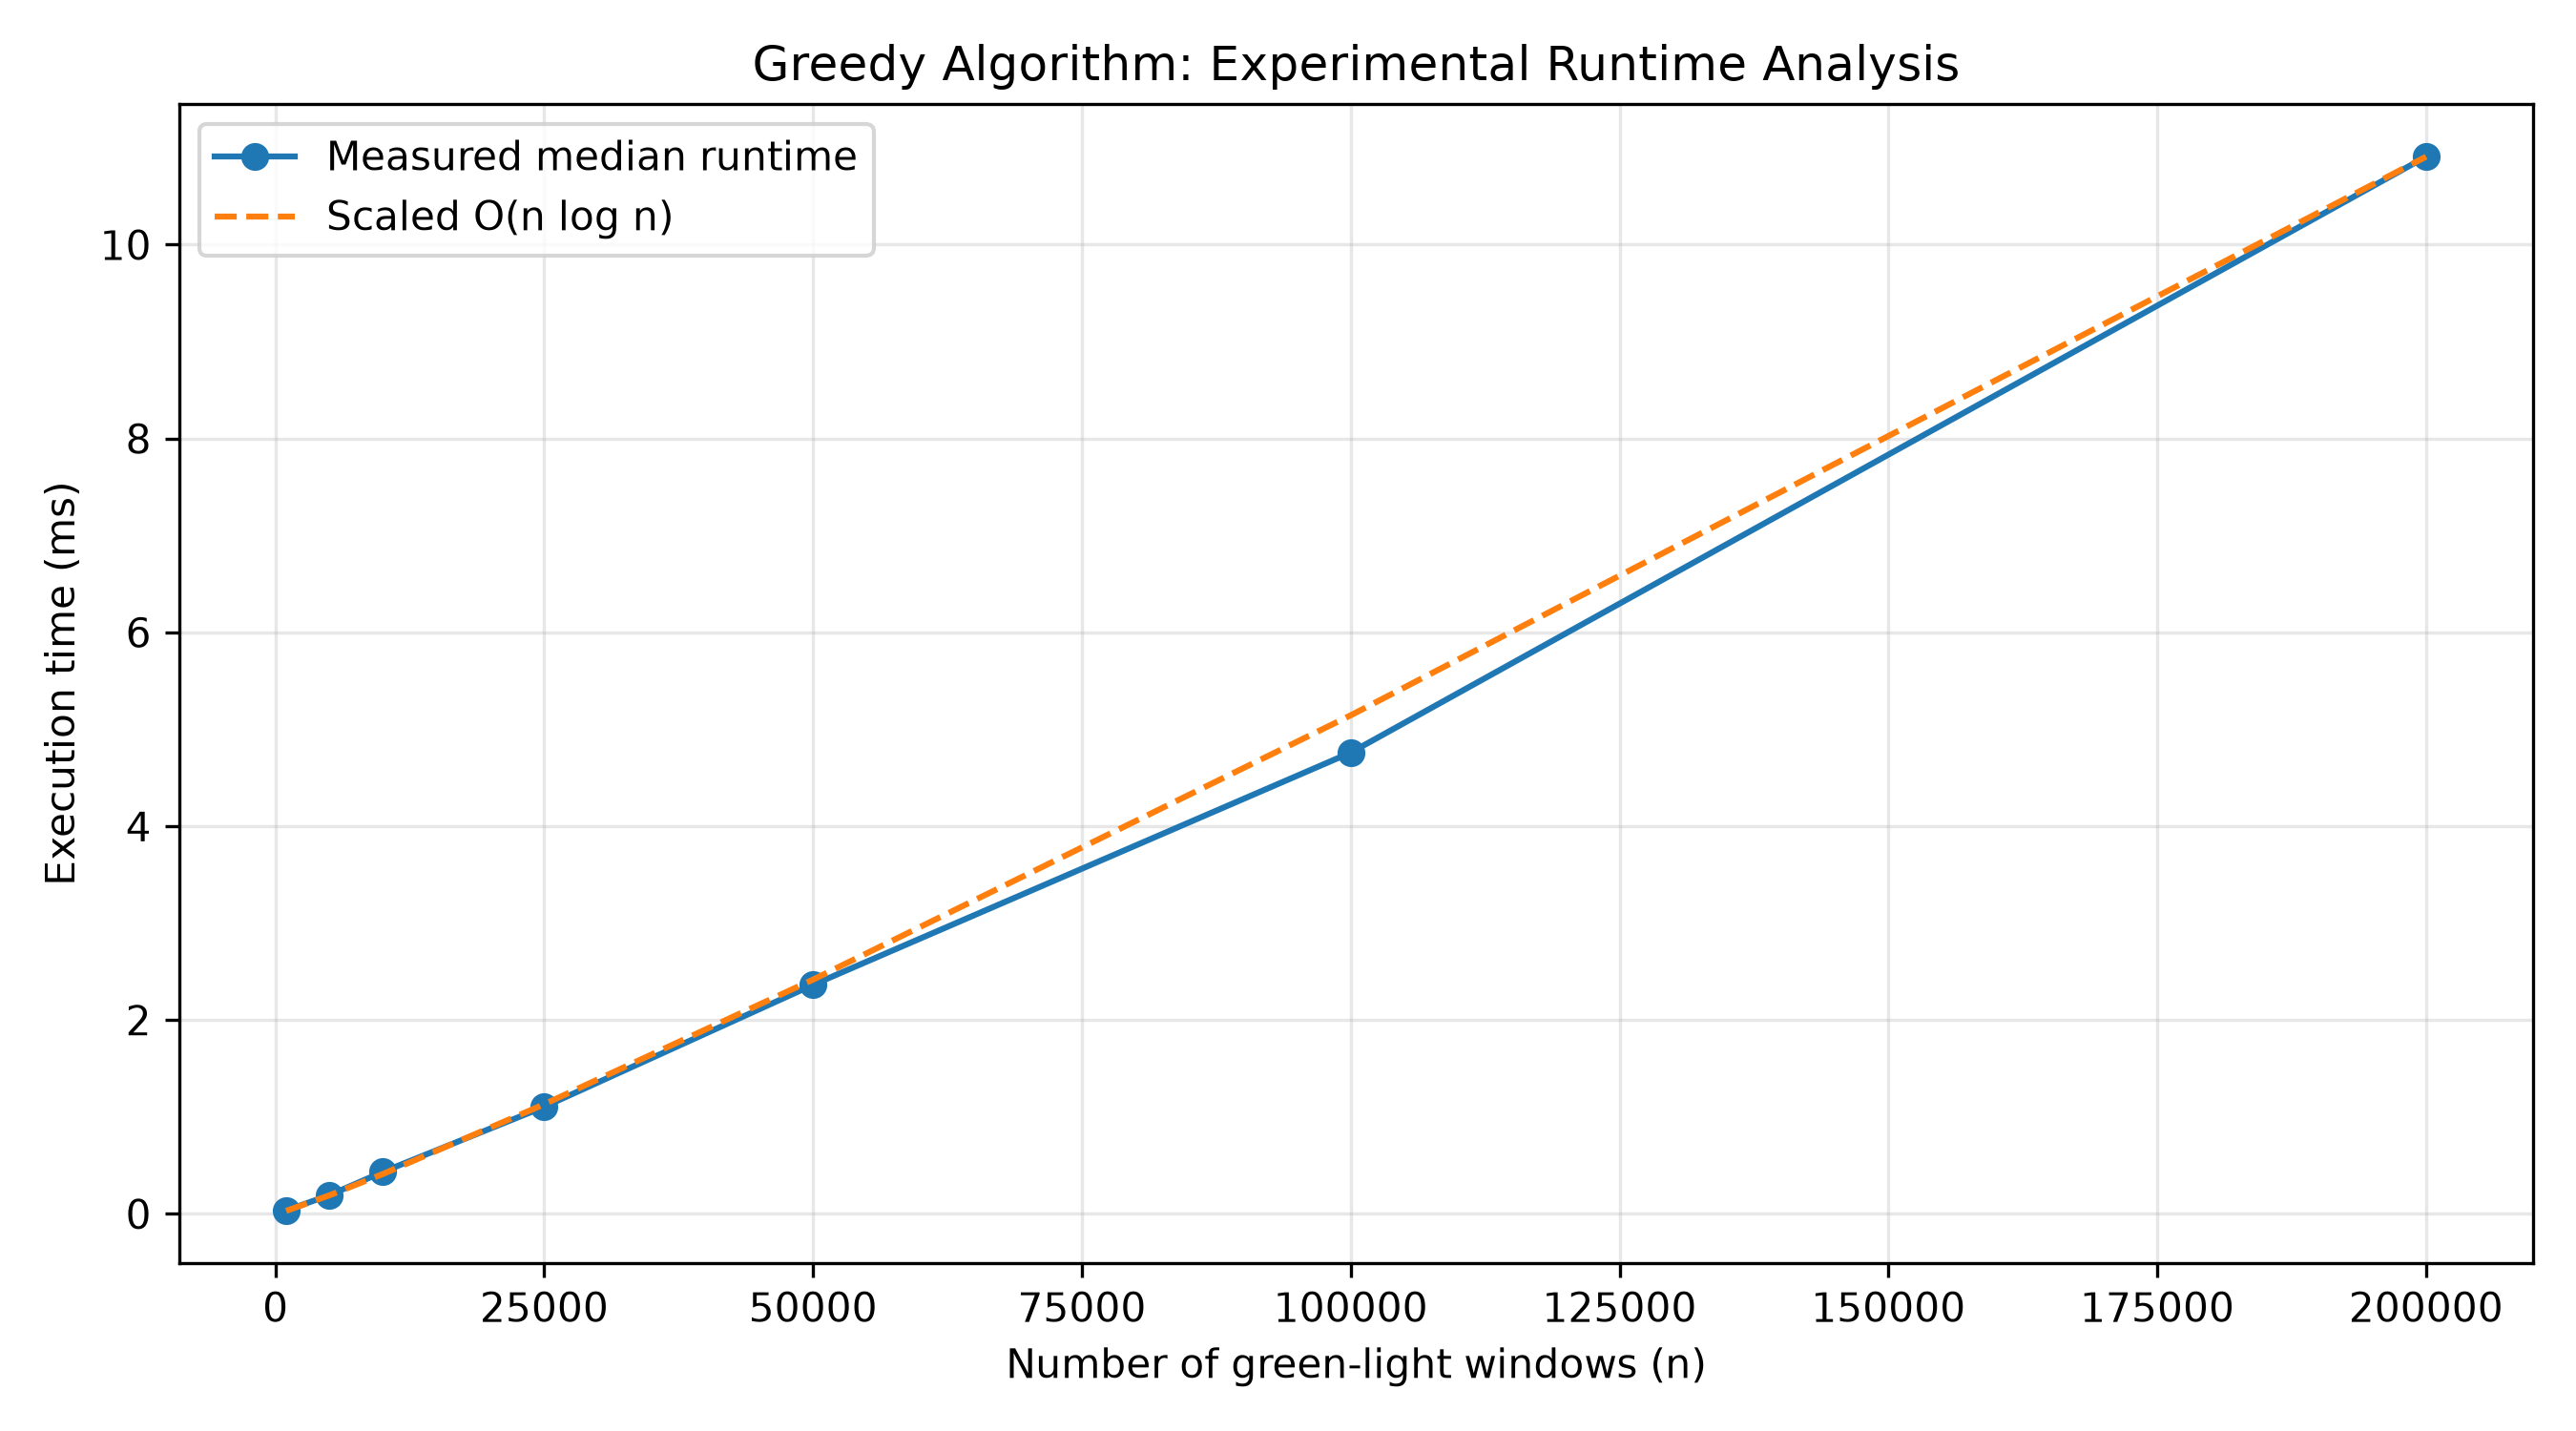
\includegraphics[width=0.9\linewidth]{runtime_graph.png}
\caption{Greedy algorithm: measured median time vs.\
scaled $O(n\log n)$ growth.}
\label{fig:greedy-runtime}
\end{figure}


% =====================================
% DIVIDE AND CONQUER
% =====================================

\section{Divide and Conquer:
Worst Queue Build-Up at an Intersection}

\subsection{Real-World Problem Description}

Signalized intersections are typically retimed
based on when and how severely queues build up
on their approaches. Traffic engineers
commonly study queues using input--output
(cumulative arrival and departure) analysis:
the number of vehicles waiting on an approach
grows when more vehicles arrive than the signal
discharges, and shrinks otherwise
\cite{daganzo1997, hcm2022}.

Modern intersections are instrumented with
vehicle detectors that report, for every short
time bin (for example, one minute), how many
vehicles arrived at the stop line and how many
departed through it. Over days or weeks of
operation this produces a long sequence of
per-minute counts.

A natural question for a traffic engineer is:
\emph{during which continuous period did the
queue on this approach grow the most?}
This period is the worst congestion episode
in the data. Identifying it tells the engineer
when the current signal timing is least able to
serve demand, and is therefore a candidate
period for retiming or coordination
\cite{fhwa2008}.

The period of interest need not align with
fixed boundaries such as the morning peak hour;
it can start and end at any minute. Short
intervals in which the queue partially drains
may lie inside the worst episode, as long as
the overall build-up across the period is
maximal.

This simplified model assumes that detector
counts are accurate, that a single approach is
studied independently, that time is divided
into equal-length bins, and that the queue is
not bounded by physical storage capacity.
The model identifies the worst episode; it does
not by itself prescribe a new signal plan.

\subsection{Mathematical Abstraction}

Let the observation horizon consist of $n$
consecutive minutes. For minute $i$, let
$a_i$ be the number of arrivals and $d_i$ the
number of departures. The net queue change in
minute $i$ is

\[
x_i = a_i - d_i \in \mathbb{Z}.
\]

The problem is therefore abstracted as a
sequence

\[
X = \langle x_1, x_2, \ldots, x_n \rangle,
\]

where $x_i > 0$ means the queue grew and
$x_i < 0$ means the queue drained.

A candidate period is a contiguous index
interval $[l, r]$ with $1 \le l \le r \le n$.
Let

\[
\mathcal{I}_n = \{ [l, r] : 1 \le l \le r \le n \}
\]

be the set of all candidate periods, so
$|\mathcal{I}_n| = n(n+1)/2$.

The total queue build-up over a period is

\[
S(l, r) = \sum_{k=l}^{r} x_k ,
\]

which, under the input--output model, equals
the difference between the queue length at the
end of minute $r$ and at the start of minute $l$.

The goal is to find

\[
[l^*, r^*] \in \arg\max_{[l,r] \in \mathcal{I}_n} S(l, r).
\]

This is the \emph{maximum subarray} problem
\cite{bentley1984, clrs2009}. Periods are
required to be non-empty; if every $x_i$ is
negative, the answer is the single minute with
the smallest drain.

\subsection{Divide-and-Conquer Algorithm Design}

The algorithm follows the divide-and-conquer
approach described by Bentley \cite{bentley1984}
and Cormen et al.\ \cite{clrs2009}.

Given the subsequence $x_{lo}, \ldots, x_{hi}$,
let $mid = \lfloor (lo + hi)/2 \rfloor$.
Every period $[l, r]$ inside $[lo, hi]$ falls
into exactly one of three cases:

\begin{enumerate}
    \item it lies entirely in the left half,
    $lo \le l \le r \le mid$;

    \item it lies entirely in the right half,
    $mid + 1 \le l \le r \le hi$;

    \item it crosses the midpoint,
    $l \le mid < r$.
\end{enumerate}

The first two cases are solved recursively.
The third case is solved directly in linear
time by the subroutine \textsc{Max-Crossing},
and the best of the three answers is returned.

\subsubsection{Algorithm Pseudocode}

\begin{verbatim}
MAX-CROSSING(X, lo, mid, hi)

1.  leftSum = -infinity;  sum = 0
2.  for i = mid downto lo:
3.      sum = sum + X[i]
4.      if sum > leftSum:
5.          leftSum = sum;  bestL = i
6.  rightSum = -infinity;  sum = 0
7.  for j = mid+1 to hi:
8.      sum = sum + X[j]
9.      if sum > rightSum:
10.         rightSum = sum;  bestR = j
11. return (bestL, bestR,
            leftSum + rightSum)

MAX-SUBARRAY(X, lo, hi)

1.  if lo == hi:
2.      return (lo, hi, X[lo])
3.  mid = floor((lo + hi) / 2)
4.  L = MAX-SUBARRAY(X, lo, mid)
5.  R = MAX-SUBARRAY(X, mid+1, hi)
6.  C = MAX-CROSSING(X, lo, mid, hi)
7.  return the one of L, R, C with
       the largest sum
       (ties: prefer L, then R)
\end{verbatim}

The initial call is
\textsc{Max-Subarray}$(X, 1, n)$.

\subsubsection{Divide, Conquer, and Combine}

\begin{itemize}
    \item \textbf{Divide:} split the horizon at
    its middle minute, in $O(1)$ time.

    \item \textbf{Conquer:} recursively find the
    worst episode within each half.

    \item \textbf{Combine:} find the worst episode
    that spans the split point and return the
    best of the three candidates, in $O(n)$ time.
\end{itemize}

\subsubsection{Explanation in the Traffic Domain}

The traffic engineer begins with the full record
of per-minute net queue changes for an approach.

Rather than examining every possible start and
end minute, which would require considering
$n(n+1)/2$ periods, the record is split into an
earlier half and a later half.

The worst congestion episode is either completely
in the earlier half, completely in the later half,
or it straddles the boundary between them.
The first two possibilities are the same question
asked about a shorter record, so the same procedure
is applied to each half until single minutes remain.

For an episode that straddles the boundary, the
engineer walks backward from the boundary and
records the start minute that accumulates the most
queue growth up to the boundary, then walks forward
from the boundary and records the end minute that
accumulates the most growth after it. Joining these
two pieces gives the worst straddling episode.

For example, consider the following ten minutes of
detector counts on one approach:

\begin{center}
\begin{tabular}{|c|c|c|c|}
\hline
Minute & Arrivals & Departures & Net $x_i$ \\
\hline
1 & 12 & 9 & $+3$ \\
2 & 8 & 10 & $-2$ \\
3 & 14 & 9 & $+5$ \\
4 & 10 & 11 & $-1$ \\
5 & 6 & 12 & $-6$ \\
6 & 13 & 9 & $+4$ \\
7 & 16 & 9 & $+7$ \\
8 & 7 & 10 & $-3$ \\
9 & 15 & 9 & $+6$ \\
10 & 4 & 12 & $-8$ \\
\hline
\end{tabular}
\end{center}

The record is split after minute 5.

\begin{itemize}
    \item The worst episode in minutes 1--5 is
    minutes 1--3, with growth $3 - 2 + 5 = 6$.

    \item The worst episode in minutes 6--10 is
    minutes 6--9, with growth
    $4 + 7 - 3 + 6 = 14$.

    \item For a straddling episode, the best start
    walking backward from minute 5 is minute 1
    (suffix sums $-6, -7, -2, -4, -1$), and the best
    end walking forward from minute 6 is minute 9
    (prefix sums $4, 11, 8, 14, 6$). The straddling
    episode, minutes 1--9, has growth $-1 + 14 = 13$.
\end{itemize}

The algorithm returns minutes 6--9: the queue on
this approach grew by 14 vehicles over those four
minutes, even though it partially drained during
minute 8. This is the period an engineer would
examine first when retiming the signal.

Note that the maximum subarray problem can also be
solved in $O(n)$ time by a scan-based method
\cite{bentley1984}. The divide-and-conquer
algorithm is studied here because it is the
technique required for this section; it also has
the practical advantage that the two halves are
independent and can be processed in parallel,
for example when detector records for different
days are stored on different machines.

\subsection{Proof of Correctness}

Throughout, for $lo \le hi$ let
$\mathcal{I}(lo, hi) = \{[l, r] : lo \le l \le r \le hi\}$
denote the set of periods inside $[lo, hi]$.

\medskip
\noindent\textbf{Lemma 1 (Crossing Periods).}
Let $lo \le mid < hi$. Then
\textsc{Max-Crossing}$(X, lo, mid, hi)$ returns
$(l', r', s')$ with $lo \le l' \le mid < r' \le hi$,
$s' = S(l', r')$, and

\[
s' = \max \{ S(l, r) : lo \le l \le mid < r \le hi \}.
\]

\noindent\textbf{Proof.}
Any crossing period $[l, r]$ splits into two
non-empty parts, $[l, mid]$ and $[mid+1, r]$, so

\[
S(l, r) = S(l, mid) + S(mid+1, r).
\]

The first term depends only on $l$ and the second
only on $r$, and every pair $(l, r)$ with
$lo \le l \le mid$ and $mid+1 \le r \le hi$ is a
valid crossing period. Hence the two terms can be
maximized independently:

\[
\max_{l, r} S(l, r)
= \max_{lo \le l \le mid} S(l, mid)
+ \max_{mid < r \le hi} S(mid+1, r).
\]

In the first loop of \textsc{Max-Crossing}, the
following invariant holds after processing index
$i$: $sum = S(i, mid)$, and $leftSum = S(bestL, mid)$
is the maximum of $S(l, mid)$ over $i \le l \le mid$.
It holds after the first iteration ($i = mid$)
because $leftSum$ starts at $-\infty$, and each later
iteration adds $X[i]$ to $sum$ and updates $leftSum$
only if the new suffix is larger. When the loop
ends at $i = lo$, $leftSum$ is the maximum over all
$lo \le l \le mid$. A symmetric invariant shows that
$rightSum$ is the maximum of $S(mid+1, r)$ over
$mid < r \le hi$. Therefore $s' = leftSum + rightSum$
is the maximum crossing sum, attained by
$[bestL, bestR]$. \hfill $\square$

\medskip
\noindent\textbf{Theorem (Correctness of Max-Subarray).}
For every $lo \le hi$,
\textsc{Max-Subarray}$(X, lo, hi)$ returns
$(l, r, s)$ with $[l, r] \in \mathcal{I}(lo, hi)$,
$s = S(l, r)$, and

\[
s = \max_{[l', r'] \in \mathcal{I}(lo, hi)} S(l', r').
\]

\noindent\textbf{Proof.}
By strong induction on the length
$m = hi - lo + 1$.

\emph{Base case} ($m = 1$). Then
$\mathcal{I}(lo, lo) = \{[lo, lo]\}$, and the
algorithm returns $(lo, lo, X[lo])$, which is the
only and therefore the best period.

\emph{Inductive step} ($m \ge 2$). Assume the
claim holds for all lengths less than $m$.
Since $lo < hi$, $mid = \lfloor (lo+hi)/2 \rfloor$
satisfies $lo \le mid < hi$, so both halves
$[lo, mid]$ and $[mid+1, hi]$ are non-empty and
have length strictly less than $m$.

The set of periods partitions as

\[
\mathcal{I}(lo, hi) = \mathcal{I}(lo, mid)
\,\cup\, \mathcal{I}(mid+1, hi)
\,\cup\, \mathcal{C},
\]

where $\mathcal{C} = \{[l, r] : lo \le l \le mid < r \le hi\}$
is the set of crossing periods. This holds because,
for any $[l, r] \in \mathcal{I}(lo, hi)$, either
$r \le mid$ (left), or $l > mid$ (right), or
$l \le mid < r$ (crossing).

By the inductive hypothesis, $L$ and $R$ are optimal
over $\mathcal{I}(lo, mid)$ and $\mathcal{I}(mid+1, hi)$,
respectively. By Lemma 1, $C$ is optimal over
$\mathcal{C}$. The maximum over a union of sets equals
the maximum of the maxima over each set, so the
candidate among $L, R, C$ with the largest sum is
optimal over $\mathcal{I}(lo, hi)$. Each of $L, R, C$
is a valid period in $\mathcal{I}(lo, hi)$ whose
reported sum equals its true sum, so the returned
triple is also valid. \hfill $\square$

\medskip
Applying the theorem with $lo = 1$ and $hi = n$
shows that the algorithm returns a period of maximum
total queue build-up over the whole observation
horizon. The algorithm terminates because each
recursive call is on a strictly shorter range.

\subsection{Running-Time Analysis}

\subsubsection{Theoretical Analysis}

Let $T(n)$ be the running time of
\textsc{Max-Subarray} on $n$ minutes of data.

For $n = 1$ the algorithm performs a constant
amount of work, so $T(1) = \Theta(1)$.

For $n \ge 2$, computing $mid$ takes $O(1)$ time,
the two recursive calls are on ranges of length
$\lceil n/2 \rceil$ and $\lfloor n/2 \rfloor$, and
\textsc{Max-Crossing} visits each of the $n$
elements of the range exactly once, taking
$\Theta(n)$ time. Choosing the best of three
candidates takes $O(1)$ time. Therefore

\[
T(n) = T(\lceil n/2 \rceil) + T(\lfloor n/2 \rfloor)
+ \Theta(n).
\]

This recurrence has the form
$T(n) = aT(n/b) + f(n)$ with $a = 2$, $b = 2$, and
$f(n) = \Theta(n) = \Theta(n^{\log_b a})$.
By case~2 of the Master Theorem
\cite[Sec.~4.5]{clrs2009} (floors and ceilings do
not affect the asymptotic solution
\cite[Sec.~4.6]{clrs2009}),

\[
\boxed{T(n) = \Theta(n \log n)}
\]

The same bound follows from the recursion tree.
The subproblems at any fixed depth are disjoint
ranges of $[1, n]$, so the crossing scans at that
depth visit at most $n$ elements in total, and the
tree has depth $\lceil \log_2 n \rceil$.
When $n$ is a power of two, every level above the
leaves visits exactly $n$ elements, so the crossing
loops perform exactly $n \log_2 n$ additions.
This count does not depend on the values $x_i$, so
the bound holds for every input, not only in the
worst case.

The recursion makes $2n - 1$ calls in total, each
doing $O(1)$ work outside the crossing loops,
contributing an additional $\Theta(n)$ term.
The extra space is $O(\log n)$ for the recursion
stack, since the algorithm works on index ranges
of the original array and never copies it.

\subsubsection{Experimental Verification}

The algorithm was implemented in C++ and tested
on randomly generated per-minute net queue changes,
drawn uniformly from $-30$ to $+30$ vehicles.

Eleven input sizes were tested, ranging from
10,000 to 16,000,000 minutes.
For each input size the measurement was repeated
10 times and the median was recorded.
Because the smallest inputs complete faster than
the resolution of the system clock, each measurement
runs the algorithm $\max(1, \lfloor 4\cdot 10^6 / n \rfloor)$
times and reports the average time per run.

Timing used the C++ \texttt{chrono} steady clock,
input generation was excluded from the timed
region, and the program was compiled with
\texttt{g++ -O2}.

Before timing, the implementation was checked
against an $O(n^2)$ brute-force search on 2,000
random inputs of length 1 to 60, and every
benchmark answer was checked against an
independent $O(n)$ scan \cite{bentley1984}.
All checks passed.

\begin{table}[htbp]
\centering
\caption{Divide-and-Conquer Running-Time Results}
\label{tab:dc-runtime}
\begin{tabular}{|r|r|r|}
\hline
Input Size ($n$) & Median Time (ms) & Time$/n$ (ns) \\
\hline
10,000 & 0.247 & 24.7 \\
20,000 & 0.553 & 27.6 \\
50,000 & 1.464 & 29.3 \\
100,000 & 2.964 & 29.6 \\
200,000 & 6.135 & 30.7 \\
500,000 & 15.607 & 31.2 \\
1,000,000 & 31.756 & 31.8 \\
2,000,000 & 64.925 & 32.5 \\
4,000,000 & 130.957 & 32.7 \\
8,000,000 & 272.306 & 34.0 \\
16,000,000 & 528.324 & 33.0 \\
\hline
\end{tabular}
\end{table}

\subsubsection{Experimental Graph}

Figure~\ref{fig:dc-runtime} (top) compares the
measured execution times with an $n\log n$ curve
scaled to match the largest input, and with the
fitted model $T(n) = a\,n\log_2 n + b\,n$.

Because $n\log n$ and $n$ differ only by a slowly
growing factor, the bottom plot shows the
normalized time $T(n)/n$ against $\log_2 n$.
If $T(n) = a\,n\log_2 n + b\,n$, this plot is a
straight line with slope $a$; a purely linear
algorithm would instead give a horizontal line.

\begin{figure}[htbp]
\centering
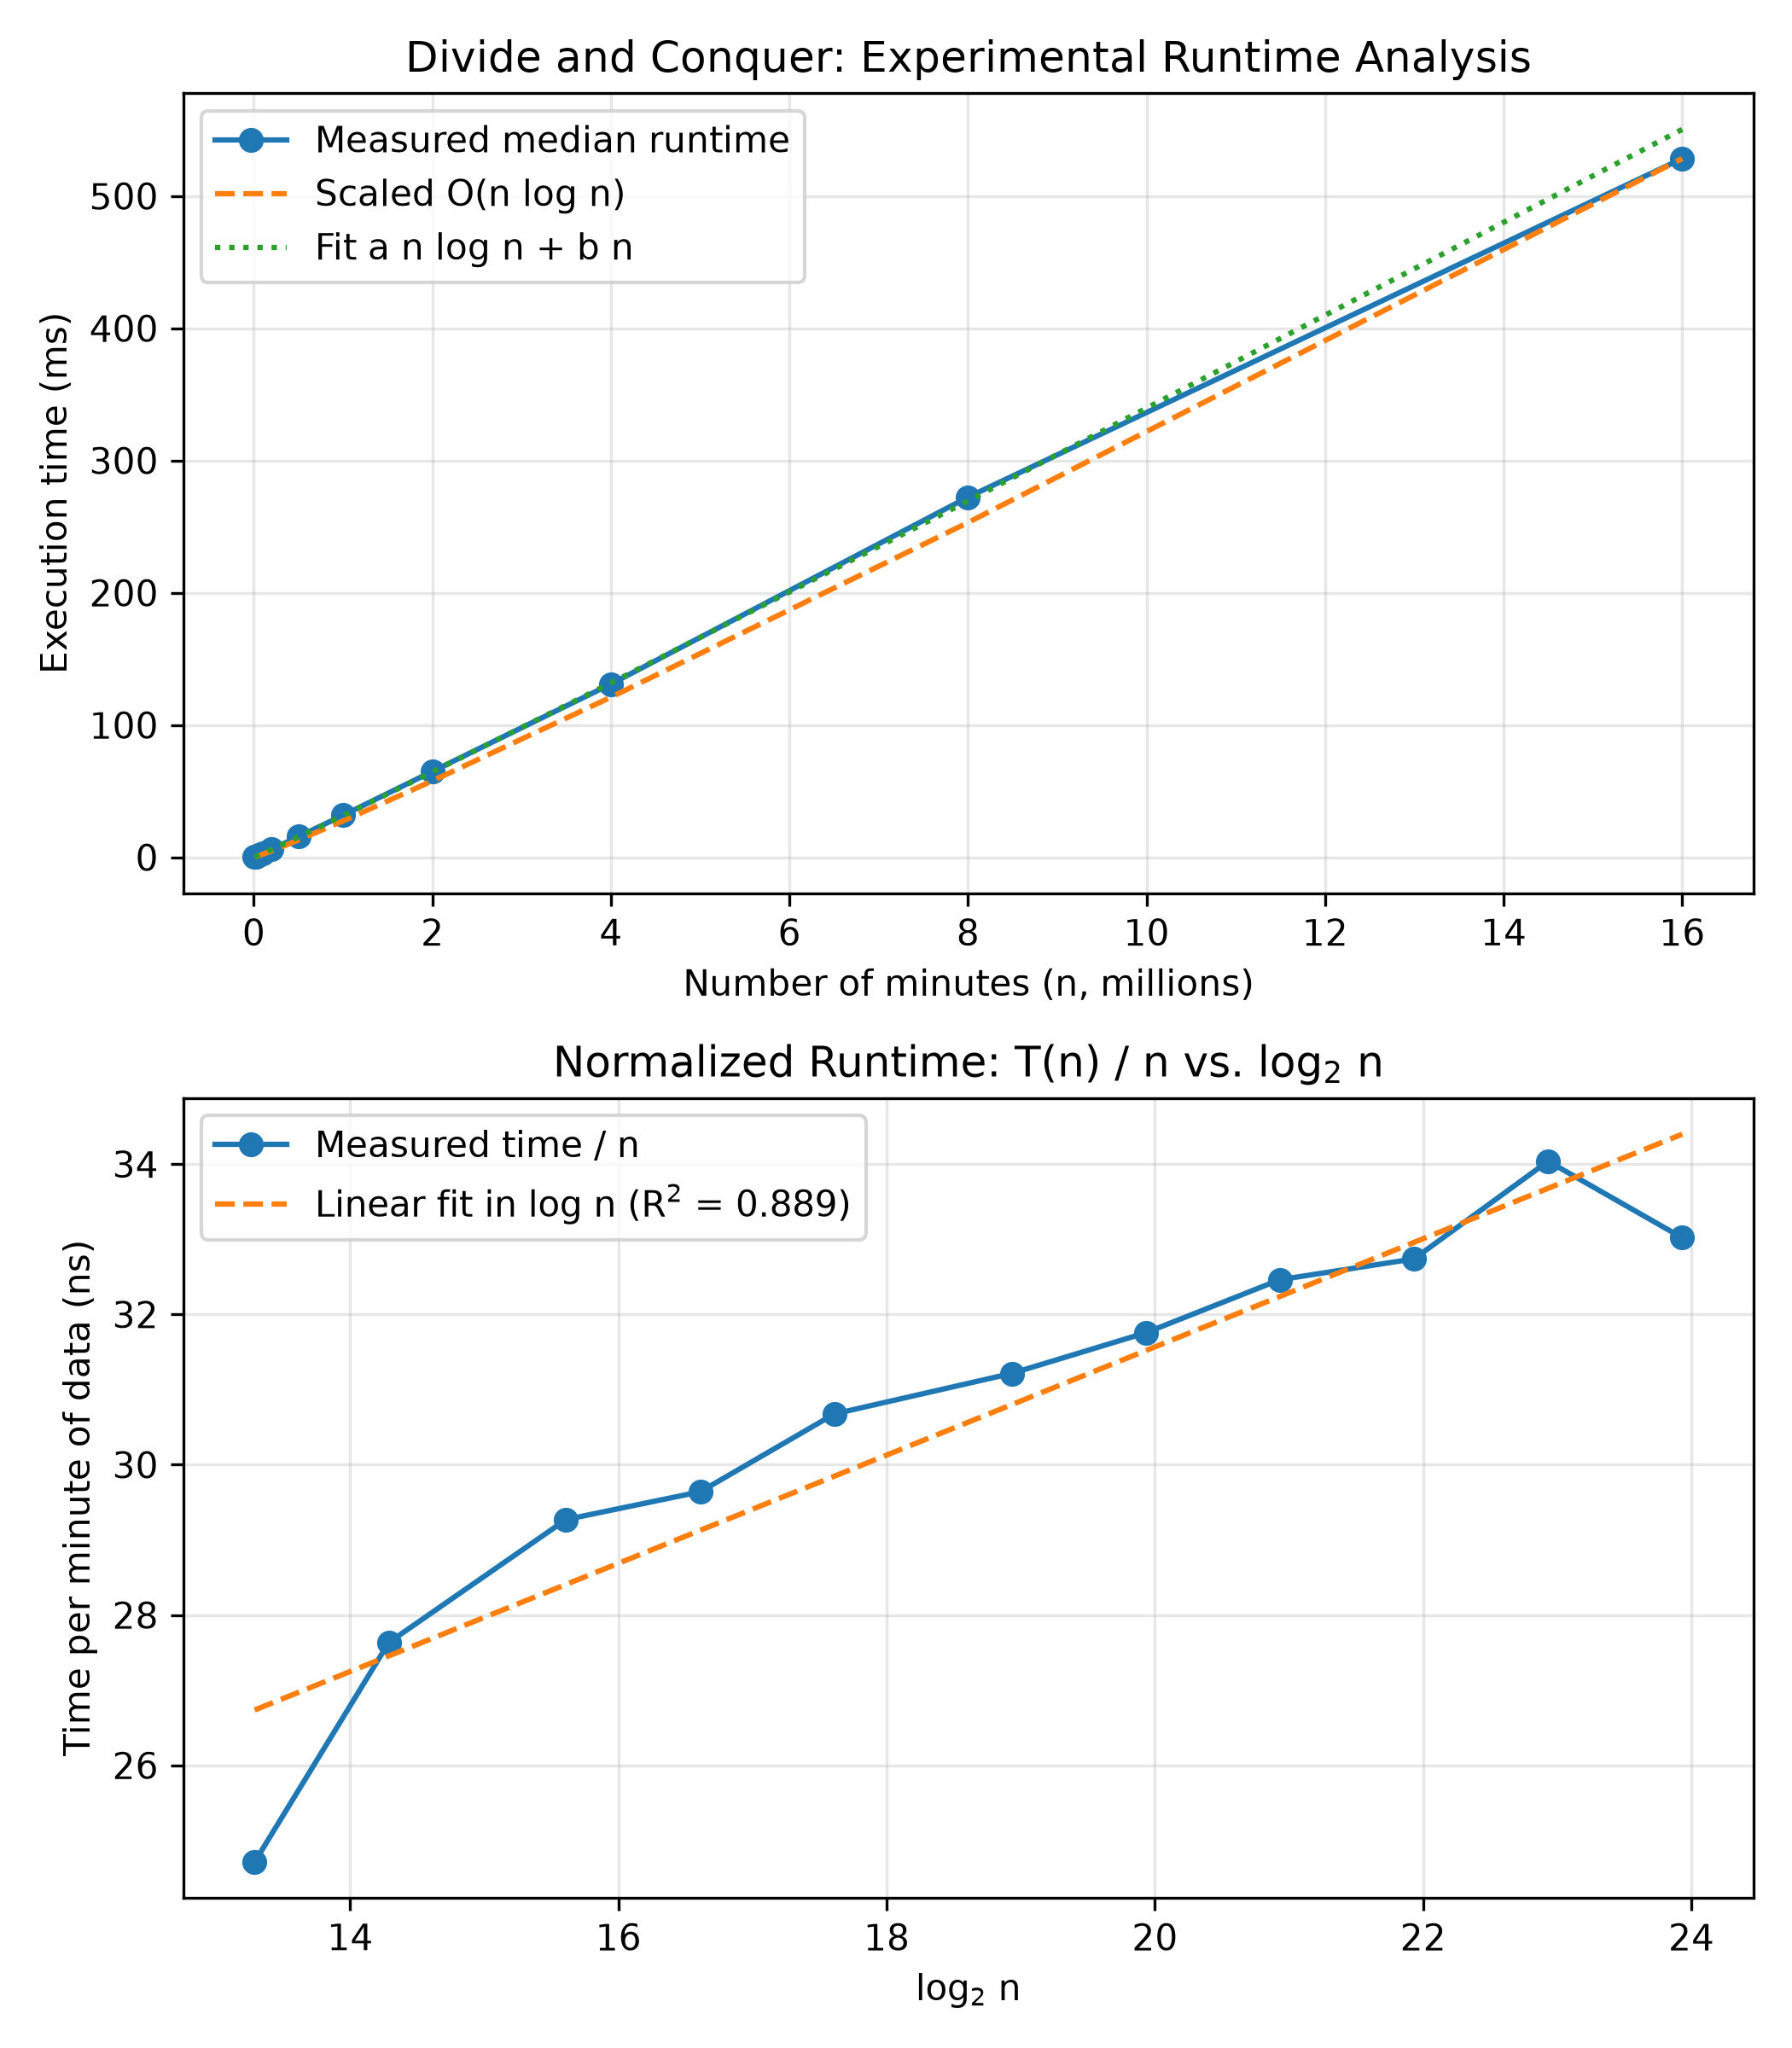
\includegraphics[width=\linewidth]{dc_runtime_graph.png}
\caption{Top: measured median execution time of
the divide-and-conquer algorithm compared with
scaled $n\log n$ growth. Bottom: time per minute
of data versus $\log_2 n$.}
\label{fig:dc-runtime}
\end{figure}

The normalized time increases steadily with
$\log_2 n$. A least-squares fit gives
$T(n)/n \approx 0.72\log_2 n + 17.2$ ns with
$R^2 = 0.889$, i.e., a positive $n\log n$
coefficient, consistent with the
$\Theta(n\log n)$ analysis.

The intercept shows that the $\Theta(n)$ term from
the $2n - 1$ recursive calls has a large constant
compared with the inexpensive additions in the
crossing loops, which is why the absolute times
in the top plot look close to linear over this
range.

Deviations from the fitted line, such as the lower
time per element at $n = 10{,}000$ (where the whole
input fits in the processor cache) and the
fluctuation at the two largest sizes, are attributed
to memory-hierarchy effects and system activity.


% =====================================
% REFERENCES
% =====================================

\bibliographystyle{IEEEtran}
\bibliography{references}

% =====================================
% APPENDICES
% =====================================

\appendices

% Greedy algorithm and experiment code
\section{Greedy Algorithm Experimental Source Code}

This appendix contains the source code used to
implement and experimentally verify the running
time of the greedy green-light window scheduling
algorithm.

The implementation uses C++17 and was tested
using the MSYS2 G++ compiler with the
\texttt{-O2} optimization flag.

\subsection{Greedy Algorithm Implementation}

Listing~\ref{lst:greedy} contains the C++
implementation of the scheduling algorithm.

\lstinputlisting[
    language=C++,
    caption={Greedy scheduling implementation},
    label={lst:greedy}
]{code/greedy.cpp}

\subsection{Experimental Runtime Measurement}

Listing~\ref{lst:experiment} contains the C++
code used to generate random intervals,
measure execution times, and calculate
median running times.

\lstinputlisting[
    language=C++,
    caption={Experimental runtime benchmark},
    label={lst:experiment}
]{code/experiment.cpp}

\subsection{Experimental Graph Generation}

Listing~\ref{lst:plot} contains the Python
code used to compare measured execution
times with theoretical $O(n\log n)$ growth.

\lstinputlisting[
    language=Python,
    caption={Python runtime graph generation},
    label={lst:plot}
]{code/plot_results.py}

% Divide-and-conquer algorithm and experiment code
\section{Divide-and-Conquer Experimental Source Code}

This appendix contains the source code used to
implement and experimentally verify the running
time of the divide-and-conquer worst queue
build-up algorithm.

The implementation uses C++14 and was tested
using the MinGW G++ compiler with the
\texttt{-O2} optimization flag.

\subsection{Divide-and-Conquer Implementation}

Listing~\ref{lst:dc-header} contains the C++
implementation of the algorithm, shared by the
demonstration program and the benchmark.

\lstinputlisting[
    language=C++,
    caption={Divide-and-conquer maximum subarray (max\_subarray.h)},
    label={lst:dc-header}
]{code/max_subarray.h}

Listing~\ref{lst:dc-demo} runs the algorithm on
the ten-minute traffic example.

\lstinputlisting[
    language=C++,
    caption={Traffic example demonstration},
    label={lst:dc-demo}
]{code/dc_max_subarray.cpp}

\subsection{Experimental Runtime Measurement}

Listing~\ref{lst:dc-experiment} contains the C++
code used to check correctness, generate random
inputs, measure execution times, and calculate
median running times.

\lstinputlisting[
    language=C++,
    caption={Divide-and-conquer runtime benchmark},
    label={lst:dc-experiment}
]{code/dc_experiment.cpp}

\subsection{Experimental Graph Generation}

Listing~\ref{lst:dc-plot} contains the Python
code used to compare measured execution times
with theoretical $\Theta(n\log n)$ growth.

\lstinputlisting[
    language=Python,
    caption={Python runtime graph generation},
    label={lst:dc-plot}
]{code/dc_plot_results.py}


% AI disclosure
\section{AI Tool Usage and Disclosure}

\subsection{AI Tool Used}

OpenAI ChatGPT was used during the development,
testing, mathematical analysis, and documentation
of the greedy traffic signal scheduling algorithm.

AI assistance included problem formulation,
algorithm explanations, C++ code generation
and revisions, debugging, experimental
benchmarking, graph generation, correctness
proofs, and LaTeX report preparation.

The following subsections summarize selected
original development interactions. These
summaries are not substitutes for the complete
conversation transcripts.

\subsection{Development and Verification}

ChatGPT assisted with algorithm design, code
revisions, debugging, and report preparation.

During debugging, complete updated code was
sometimes requested so that suggested corrections
could be applied consistently instead of making
individual line-by-line edits.

The C++ implementation was compiled and tested.
Runtime experiments were executed, and the
recorded measurements were used to generate
the experimental graph.

The project models maximum-cardinality interval
scheduling using preapproved green-light windows.
It does not claim to minimize actual traffic
congestion or vehicle waiting times.

\subsection{Problem Selection and Abstraction}

\noindent\textbf{Original User Prompt:}

\begin{quote}
what if i change it to the max amount of time
you can have lights running at the same time
to avoid cloging traffic
\end{quote}

\noindent\textbf{AI-Generated Result Summary:}

ChatGPT discussed traffic signal coordination
and suggested modeling the problem as
maximum-cardinality interval scheduling.

The objective was to select the maximum number
of mutually compatible green-light windows,
not to directly minimize traffic congestion.

\subsection{Greedy Algorithm Implementation}

\noindent\textbf{Original User Prompt:}

\begin{quote}
okay lets se
\end{quote}

\noindent\textbf{AI-Generated Result Summary:}

ChatGPT explained the earliest-finish-time
greedy algorithm and provided C++ implementation
assistance.

The algorithm sorts candidate windows by
finishing time and selects windows that do not
overlap previously selected windows.

\subsection{Code Review and Debugging}

\noindent\textbf{Original User Prompt:}

\begin{quote}
before i push it chekc my code correct what
needs to be correctedso i know im pushing
the full correct file
\end{quote}

\noindent\textbf{AI-Generated Result Summary:}

ChatGPT reviewed the C++ implementation,
identified possible corrections, and provided
suggestions for initialization, output formatting,
and code organization.

\subsection{Experimental Runtime Analysis}

\noindent\textbf{Original User Prompt:}

\begin{quote}
give me the whole code
\end{quote}

\noindent\textbf{AI-Generated Result Summary:}

ChatGPT provided a complete C++ benchmarking
program for generating random candidate windows
and measuring the greedy algorithm's running time.

Seven input sizes from 1,000 to 200,000 windows
were tested. Each size used ten repetitions,
and median execution times were recorded.

The measurements were compared against
the theoretical $O(n\log n)$ running time.

\subsection{Experimental Graph Generation}

\noindent\textbf{Original User Prompt:}

\begin{quote}
so run this python Greedy/plot\_results.py
\end{quote}

\noindent\textbf{AI-Generated Result Summary:}

ChatGPT assisted with executing the Python
plotting program, reading CSV data, correcting
file and column naming issues, and generating
the experimental runtime graph.

\subsection{Correctness Proof}

\noindent\textbf{Original User Prompt:}

\begin{quote}
so show me exactly what i should write
\end{quote}

\noindent\textbf{AI-Generated Result Summary:}

ChatGPT provided a LaTeX correctness proof
using the exchange-argument technique.

The proof explains why selecting the
earliest-finishing compatible window preserves
an optimal solution and why the argument can
be repeated for the remaining intervals.

\subsection{LaTeX Report Assistance}

\noindent\textbf{Original User Prompt:}

\begin{quote}
so write me the greedy\_runtime.text
and i thought therw was an ai usage apendix
\end{quote}

\noindent\textbf{AI-Generated Result Summary:}

ChatGPT assisted with runtime analysis,
experimental results, graph inclusion,
source-code listings, AI disclosure,
and IEEE conference-style formatting.

\subsection{Verification and Experimental Results}

The greedy implementation was compiled
and tested using the MSYS2 G++ compiler.

The runtime experiment used the
\texttt{-O2} compiler optimization flag.

Seven input sizes were evaluated using
ten timing measurements per input size.

Median execution times were saved to CSV
and visualized using Python and Matplotlib.

The measured results were consistent with
the theoretical $O(n\log n)$ running time.

\subsection{Complete AI Interaction Record}

The preceding subsections document selected
original AI prompts and summarize their results.

The complete original project-development
conversation was recovered from the ChatGPT
data export. It contains the original prompts,
responses, intermediate code revisions,
debugging discussions, and documentation
assistance.

The original conversation is reproduced
in the following appendix.

Seven additional revised AI interactions,
including their prompts and responses,
are reproduced in a separate appendix.

OpenAI ChatGPT was the AI tool used for
the greedy algorithm portion of this project.

% Complete original ChatGPT conversation

\clearpage
\section{Selected Original AI Development Interactions}

\noindent\textbf{AI Tool:} OpenAI ChatGPT

This appendix presents ten selected interactions
from the original project-development conversation.
The questions were selected to document important
decisions, technical questions, debugging, and
verification during the greedy algorithm project.

The responses below are concise summaries of the
original AI-generated results, rather than verbatim
reproductions of the complete responses.

\subsection{Traffic Signal Problem Selection}

\noindent\textbf{User Prompt:}

\begin{quote}
what if i change it to the max amount of time
you can have lights running at the same time
to avoid cloging traffic
\end{quote}

\noindent\textbf{Result Summary:}

ChatGPT discussed traffic signal coordination
and proposed a simplified problem involving
nonoverlapping green-light time windows.

\subsection{Understanding the Greedy Objective}

\noindent\textbf{User Prompt:}

\begin{quote}
we want mutiple windos and by selecting one
big one it doesnt match our greedy stratagy
\end{quote}

\noindent\textbf{Result Summary:}

ChatGPT explained why maximizing the number
of compatible windows differs from selecting
the window with the longest duration.

\subsection{Understanding Sorting}

\noindent\textbf{User Prompt:}

\begin{quote}
so what we just did is sort the window sto
get the correct windows or were doing that
right nwo
\end{quote}

\noindent\textbf{Result Summary:}

ChatGPT explained the difference between
sorting by finishing time and selecting
compatible windows using the greedy rule.

\subsection{Scheduling Accuracy}

\noindent\textbf{User Prompt:}

\begin{quote}
what if the timeings off it willl throw
everythingoff
\end{quote}

\noindent\textbf{Result Summary:}

ChatGPT discussed scheduling assumptions,
timing compatibility, and the limitations
of applying this simplified algorithm
to actual traffic signals.

\subsection{Experimental Implementation}

\noindent\textbf{User Prompt:}

\begin{quote}
give me the whole code
\end{quote}

\noindent\textbf{Result Summary:}

ChatGPT provided implementation assistance
for measuring the greedy algorithm's
execution time using C++.

\subsection{Benchmark Debugging}

\noindent\textbf{User Prompt:}

\begin{quote}
send me the updated experiment code so i
can just paste itbecause imgetting errors
\end{quote}

\noindent\textbf{Result Summary:}

ChatGPT assisted with correcting the
experimental benchmarking program,
including runtime measurements and
CSV result generation.

\subsection{Experimental Graph}

\noindent\textbf{User Prompt:}

\begin{quote}
so run this python
\texttt{Greedy/plot\_results.py}
\end{quote}

\noindent\textbf{Result Summary:}

ChatGPT assisted with executing the
Python graph-generation script and
visualizing measured execution times
against theoretical growth.

\subsection{Correctness Proof}

\noindent\textbf{User Prompt:}

\begin{quote}
so show me exactly what i should write
\end{quote}

\noindent\textbf{Result Summary:}

ChatGPT provided LaTeX assistance for
the correctness proof, explaining the
exchange argument that establishes
the greedy algorithm's optimality.

\subsection{Reviewing Project Progress}

\noindent\textbf{User Prompt:}

\begin{quote}
okay give me a recap on wat i justdid
and a recap on what i did and need to
do to complete this project
\end{quote}

\noindent\textbf{Result Summary:}

ChatGPT reviewed completed development
work and identified remaining report,
experimental, and documentation tasks.

\subsection{AI Documentation Requirements}

\noindent\textbf{User Prompt:}

\begin{quote}
okay so what am i missing for the ai
part like how do i complete it
\end{quote}

\noindent\textbf{Result Summary:}

ChatGPT explained the AI-disclosure
requirements and discussed recording
prompts, responses, and intermediate
results in a LaTeX appendix.

\subsection{Original Transcript Preservation}

The preceding entries represent selected
interactions from the original conversation.

The complete original conversation,
including all intermediate prompts,
responses, code, and debugging records,
is retained in the project repository
as a separate text file.

These summaries do not replace the full
interaction records required by the
assignment instructions.


% Seven revised AI interactions
\section{Revised AI Interactions}

Seven additional ChatGPT interactions (October 19,
2026) were used to review and document the greedy
project. Each entry gives the exact prompt and a
summary of the response.

\begin{enumerate}

\item \textbf{Problem selection and abstraction.}
\emph{Prompt:} ``I am completing a graduate-level
Analysis of Algorithms project that requires a
real-world application of a greedy algorithm. I want
to investigate traffic signal scheduling to help avoid
overlapping green-light opportunities and potentially
reduce scheduling conflicts. Can you explain how to
formulate a simplified traffic signal scheduling
problem using interval scheduling? Define the candidate
green-light windows, starting and finishing times,
compatibility constraints, objective function,
assumptions, and limitations. Clearly distinguish
maximizing the number of compatible windows from
minimizing actual traffic congestion.''
\emph{Result:} Defined windows $w_i=(s_i,f_i)$, the
compatibility condition $f_i \le s_j$, and the
objective $\max|S|$; listed the model's assumptions;
and explained that it maximizes compatible windows
rather than minimizing congestion.

\item \textbf{Greedy algorithm and C++ implementation.}
\emph{Prompt:} ``For my COT5405 Analysis of Algorithms
project, I modeled traffic signal scheduling as a
maximum-cardinality interval scheduling problem. Each
candidate green-light window has an ID, start time, and
finish time. Explain the earliest-finish-time greedy
algorithm step by step, provide pseudocode, and show a
complete C++17 implementation using a struct, vector,
and std::sort. Use the example windows (1,0,10),
(2,2,5), (3,5,8), (4,7,12), and (5,8,14). Explain why
the selected windows are 2, 3, and 5.''
\emph{Result:} Provided pseudocode, a C++17
implementation, a walkthrough selecting windows 2, 3,
and 5, and an $O(n\log n)$ analysis.

\item \textbf{Code review and debugging.}
\emph{Prompt:} ``I have written a C++17 greedy algorithm
to select the maximum number of mutually compatible
green-light windows. Review my implementation for
correctness, compilation errors, sorting logic,
boundary conditions, and output formatting. Explain
every necessary correction and why it matters. Preserve
my original program structure as much as possible
instead of rewriting the entire implementation. Also
identify useful test cases, including overlapping
intervals, back-to-back intervals, empty input, and
intervals with identical finishing times. Here is my
implementation:'' [followed by the complete 25-line
\texttt{greedy.cpp} program, omitted here for space]
\emph{Result:} Confirmed the code was correct for the
example; noted that initializing \texttt{lastFinish} to
$-1$ assumes nonnegative start times and suggested a
generalization; proposed edge-case tests.

\item \textbf{Experimental runtime analysis.}
\emph{Prompt:} ``I need to experimentally verify the
O(n log n) running-time complexity of my C++
earliest-finish-time greedy interval scheduling
algorithm. Help me design and implement a C++17
benchmark that generates random green-light windows for
input sizes 1,000, 5,000, 10,000, 25,000, 50,000,
100,000, and 200,000. Use a fixed random seed for
reproducibility, run 10 repetitions per input size,
measure sorting and greedy selection using
std::chrono::steady\_clock, exclude input generation
from the timed section, compute median execution time
in milliseconds, and export InputSize, MedianTimeMs, and
NLogN to Greedy/results.csv. Explain compilation using
g++ -std=c++17 -O2 and the limitations of runtime
measurements.''
\emph{Result:} Provided the benchmark in
Listing~\ref{lst:experiment} (seed 42, median of ten
runs, CSV export) and discussed measurement noise.

\item \textbf{Runtime graph generation.}
\emph{Prompt:} ``I have a CSV file at Greedy/results.csv
containing the columns InputSize, MedianTimeMs, and
NLogN from my C++ greedy algorithm benchmark. Show me
how to write and execute Greedy/plot\_results.py using
Python, csv.DictReader, and Matplotlib. Plot measured
median execution time against input size and compare it
with a scaled theoretical n log2(n) curve. Save the
figure as Greedy/runtime\_graph.png. Explain the meaning
of the graph, how it supports the theoretical runtime
analysis, and how to diagnose incorrect CSV headers or
missing files.''
\emph{Result:} Provided the plotting script
(Listing~\ref{lst:plot}), explained scaling the
$n\log_2 n$ curve to the largest measurement, and
described common file and header errors.

\item \textbf{Correctness proof.}
\emph{Prompt:} ``I need a formal proof of correctness for
the earliest-finish-time greedy algorithm used in my
traffic signal scheduling project. The objective is to
maximize the number of nonoverlapping candidate
green-light windows, where each window has a start and
finish time and two consecutive windows are compatible
if the next starts at or after the previous finishes.
Provide a clear theorem and an exchange-argument proof
showing why replacing the first interval of an optimal
schedule with the earliest-finishing interval preserves
optimality. Explain why the argument can be applied
repeatedly to the remaining intervals. Provide the
proof in LaTeX and state its assumptions.''
\emph{Result:} Gave a theorem and exchange-argument
proof, completed by induction on the number of windows.

\item \textbf{Report preparation and AI disclosure.}
\emph{Prompt:} ``I am preparing a COT5405 algorithms
group project report in Overleaf using the IEEE
conference template. My portion covers greedy traffic
signal window scheduling. Help me organize the report
into a real-world problem description, mathematical
abstraction, algorithm and pseudocode, correctness
proof, theoretical O(n log n) analysis, empirical
runtime table and graph, bibliography, and source-code
appendix. Explain how to divide sections into separate
LaTeX files using input commands, include a PNG figure,
include C++ and Python code using the listings package,
and use BibTeX. Also help me prepare a transparent AI-use
appendix distinguishing exact original prompts and
responses from summaries or newly generated
interactions. My partner's divide-and-conquer section
will be added later.''
\emph{Result:} Proposed the IEEE report structure and
\texttt{\textbackslash input} file layout, showed how to
include figures, code listings, and BibTeX references,
and advised keeping original and revised AI records
separate.

\end{enumerate}


\end{document}
